\section{Introduction}

Medicine has a procedure for a hard case: convene several specialists, let each form a view, and
see whether the views agree. Clinicians trained differently make different mistakes, so agreement
on a diagnosis provides corroborating evidence. That is why a tumour board's agreement informs a
treatment decision and why a matching second opinion supports the initial diagnosis.

\begin{figure*}[t]\centering
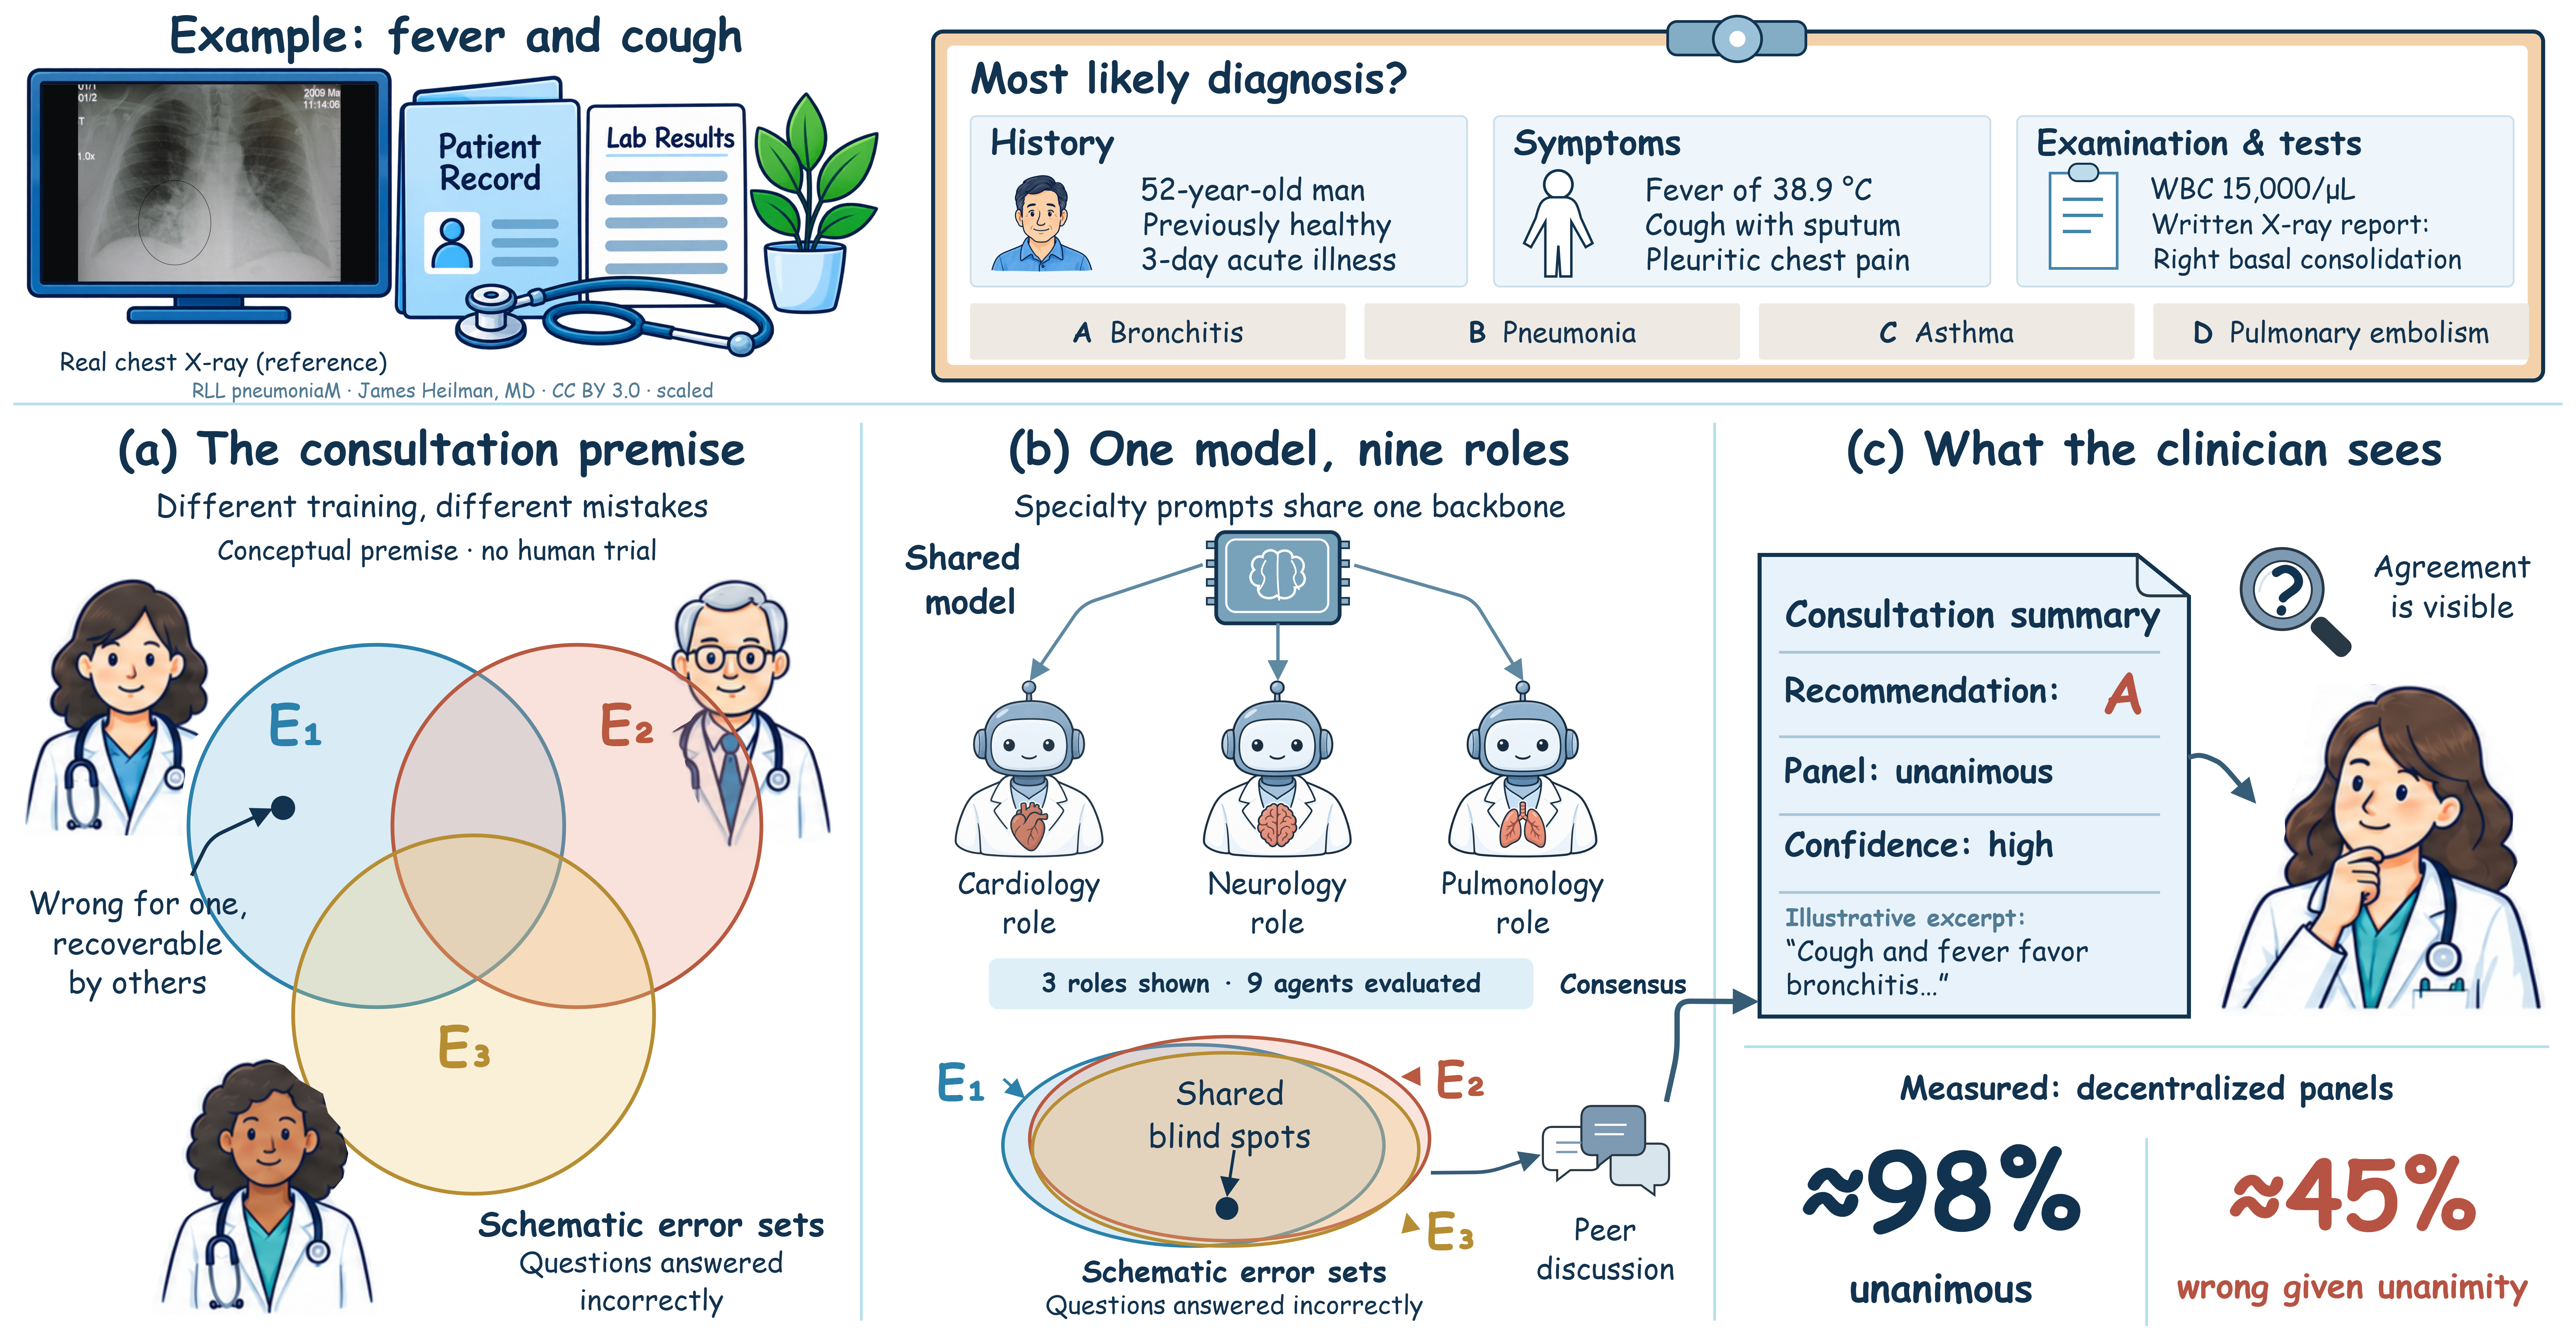
\includegraphics[width=\textwidth]{figures/figure-1.png}
\caption{\textbf{A panel that agrees is not a panel that knows.} The top row illustrates a case; B is correct. (a) Differently trained clinicians correct each other's errors. (b) Role-prompted agents' shared blind spots become consensus through discussion. (c) Clinicians receive a unanimous, high-confidence wrong recommendation. Decentralized panels ($N{=}9$) are $98.0\%$ unanimous; $44.9\%$ of unanimous answers are wrong (Table~\ref{tab:safety}).}
\label{fig:teaser}
\end{figure*}

Multi-agent consultation transplants the procedure into language-model systems.
MedAgents~\citep{tang2024medagents}, MDAgents~\citep{kim2024mdagents}, MAC~\citep{chen2025mac} and
TeamMedAgents~\citep{teammedagents} build the same object: several agents prompted into clinical
specialties, discussing cases until they agree, on the reasoning that a panel of specialists
diagnoses better than the single doctor. This reasoning requires the specialists to make
different mistakes: pooling correlated judgements repeats them rather than combining
them~\citep{kurvers2016boosting, kammer2017}. Figure~\ref{fig:teaser} contrasts this independence
premise with the behaviour of role-prompted panels.

In this work we measure it. A consultation is worth assembling only if somebody in the room is
right when the others are wrong, and the room can tell who. We measure headroom and capture rate
$\kappa$; collaboration gain is exactly their product. Our evaluation covers $480$ multi-agent
configurations and $161{,}999$ episodes. It uses eight models from four vendors, three medical
benchmarks, four multi-agent architectures and panel sizes $N \in \{1,3,5,7,9\}$. A
budget-matched single-model control accompanies every cell.

Agents prompted into different medical specialties fail on the same items. Their pairwise error
correlation is $\varphi = 0.76$, leaving a nine-member panel with $1.27$ effective independent
opinions. Peer discussion raises the correlation to $0.990$, leaving $1.01$ effective opinions.
Computed from raw $\varphi$, mixing model generations within one vendor yields $2.60$ effective
opinions in a nine-member panel; mixing models from six vendors yields $2.29$.

Run from their own repositories on the same items with \texttt{gpt-4.1-nano},
MedAgents~\citep{tang2024medagents} and MDAgents~\citep{kim2024mdagents} gain $+5.7$ and
$+1.2$ percentage points over the single doctor, a factor of five apart. Their agents' errors
correlate at $0.860$ and $0.863$, above $0.792$ for our panels on the same model.

Selection limits the gain from this headroom. At nine agents the oracle ceiling is $63.9\%$
against $53.1\%$ for the single doctor, giving $10.7$\,pp of headroom. Across the four
architectures and self-consistency, capture rate $\kappa$ ranges from $-7.4\%$ for Hybrid to
$17.7\%$ for Decentralized. Two classifiers trained on fifteen first-round features against ground truth do not outperform
plurality voting.

In medicine, agreement affects safety. At $N{=}9$, discussion raises unanimity from $67.5\%$
(Independent) to $98.0\%$ (Decentralized), while the error rate among unanimous answers rises
from $38.1\%$ to $44.9\%$. Unanimity separates the panel's right answers from its
wrong ones at $\text{AUC} = 0.59$.

The rest of the paper is organised as follows. Section~\ref{sec:related} places the work against
the collective-intelligence results the design pattern borrows from and the medical systems built
on them. Section~\ref{sec:metrics} defines the two measurements and the seven conditions.
Section~\ref{sec:premise} examines error correlation and the four sources of panel diversity;
Section~\ref{sec:ceiling} measures how much headroom aggregation recovers; and
Section~\ref{sec:safety} reports the effects of consultation on agreement.
